\documentclass[10pt,a4paper]{article}
\usepackage[utf8]{inputenc}
\usepackage{amsmath}
\usepackage{amsfonts}
\usepackage{amssymb}
\usepackage{todonotes}
\usepackage{graphicx}
\usepackage[titletoc,title]{appendix}
\usepackage{hyperref}
\hypersetup{
    colorlinks,
    citecolor=black,
    filecolor=black,
    linkcolor=black,
    urlcolor=black
}

\begin{document}

\begin{titlepage}

\newcommand{\HRule}{\rule{\linewidth}{0.5mm}} % Defines a new command for the horizontal lines, change thickness here

\center % Center everything on the page
 
\textsc{\LARGE KU Leuven}\\[1.5cm] % Name of your university/college
\textsc{\Large 1 Ma Ingenieurswetenschappen: Computerwetenschappen}\\[0.5cm] % Major heading such as course name
\textsc{\large Bedrijfservaring: Computerwetenschappen}\\[0.5cm] % Minor heading such as course title


\HRule \\[0.4cm]
{ \huge \bfseries Stageverslag bedrijfservaring Alcatel-Lucent}\\[0.4cm]
\HRule \\[1.5cm]
 

\Large \emph{Author:}\\
Helena \textsc{Brekalo}\\[3cm]

{\large \today}\\[3cm] % Date

\vfill % Fill the rest of the page with whitespace

\end{titlepage}

\textbf{Gegevens student:}
Helena Brekalo\\
1e master Computerwetenschappen (Veilige software)\\
\medskip
\\
\textbf{Gegevens bedrijf:}\\
Alcatel-Lucent\\
Copernicuslaan 50\\
2018 Antwerpen\\
\medskip
\\
\textbf{Gegevens stagebegeleider:}\\
Bart Hemmeryckx-Deleersnijder\\
E-mail: bart.hemmeryckx-deleersnijder@alcatel-lucent.be\\
GSM-nummer: +32 472 95 00 65\\
Vast nummer binnen het bedrijf: +32 3 240 8525
\medskip
\\
\textbf{Stageperiode:}\\
1 juli - 7 augustus\\
7 september - 11 september
\clearpage

\begin{center}
\textbf{Samenvatting}\\
\end{center}
Dit verslag beschrijft de opgedane kennis en ervaring tijdens mijn 6 weken durende stage bij Alcatel-Lucent in Antwerpen. Het doel tijdens de stage was om een dashboard te ontwerpen en implementeren voor het continuous integration systeem Jenkins en op deze manier "Jenkins-awareness" te cre\"eren.\\
Het dashboard is ontwikkeld met Dashing en toont het overzicht van een reeks zelfgekozen builds. De ontwikkeling is gebeurd in Javascript, Coffeescript, SCSS, Ruby en HTML op Linux.\\
Gedurende de stage werd ik erg betrokken bij alle onderdelen van het scrum-proces, zodat ik me een beeld kon vormen van hoe dit er in het bedrijfsleven aan toe gaat.

\tableofcontents
\clearpage

\section{Inleiding}
De probleemstelling, waarvoor ik tijdens mijn stage een oplossing ontworpen heb, gaat als volgt. Op de afdeling Motive Network-Analyzer Copper (NA-C) bij Alcatel-Lucent in Antwerpen doet men aan continuous integration, waarbij gebruik gemaakt wordt van de tool Jenkins. Deze biedt een dashboard om het overzicht van de build statussen weer te geven, maar de software-ontwikkelaars hebben niet de neiging deze te bekijken op de televisie die aanwezig is. Het doel van mijn stage was om "Jenkins-awareness" te cre\"eren en een dashboard te ontwikkelen dat snel een overzicht toont van de builds waar aandacht aan besteed moeten worden. Op de afdeling NA-C werkt men volgens het agile-principe van scrum, waar ik zelf ook gebruik van maakte. Zo kreeg ik mijn eigen project toegewezen en moest ik tweewekelijkse sprints inplannen en evaluaties uitvoeren.\\

Om dit te realiseren, heb ik tijdens de eerste sprint een literatuurstudie uitgevoerd, om mij zo een idee te vormen van hoe het dashboard eruit moet zien. Tijdens de tweede sprint is het dashboard ontwikkeld, met behulp van Dashing. Aan het einde van de tweede sprint is deze ge\"evalueerd door middel van een demonstratie voor de teams in Antwerpen, Chennai en Bangalor. Op basis van de feedback die hierop ontvangen werd, zijn veranderingen doorgevoerd gedurende de derde sprint. In het tweede deel van de derde sprint is het dashboard in gebruik genomen op de Jenkins server van NA-C.\\

De voornaamste resultaten zijn het dashboard dat succesvol ontwikkeld is, door te werken via de scrum-methode. De talen die ik hierbij heb geleerd zijn Javascript, Coffeescript, (S)CSS, HTML en Ruby. Het dashboard is nu ook voorzien van documentatie, om hergebruik te vergemakkelijken. Doordat ik overal in betrokken werd, heb ik nu ook een idee van hoe grote projecten verlopen in een bedrijfsomgeving.\\

Dit verslag is als volgt ingedeeld. In Sectie \ref{bedrijf} wordt het bedrijf Alcatel-Lucent voorgesteld. De derde sectie behandelt de stage (Sectie \ref{stage}), waarin de afdeling waar ik gewerkt heb wordt voorgesteld (Subsectie \ref{afdeling}), er wordt uitgelegd volens welke methoden er wordt gewerkt (Subsectie \ref{methoden}). Mijn stageopdracht wordt uitgelegd in Subsectie \ref{opdracht}. Het resultaat wordt besproken in Subsectie \ref{resultaat}. Gedurende mijn stage waren er ook initiatieven voor interns, wat besproken wordt in Subsectie \ref{interns}.\\
Sectie \ref{relatie} legt de link tussen de stage en mijn opleiding. De kritische reflectie van de competenties die ik trachtte te verbeteren is te vinden in Sectie \ref{reflectie}. Sectie \ref{besluit} bevat het besluit en de appendices zijn te vinden in Appendix \ref{lit_study} en \ref{enquete1}. \todo{ref naar andere appendices toevoegen}

\section{Het bedrijf: Alcatel-Lucent}
\label{bedrijf}
Alcatel-Lucent is een Frans bedrijf met de hoofdzetel in Frankrijk en vestigingen in Amerika, Azi\"e, het Midden-Oosten, Afrika en Europa, waaronder een vestiging in Antwerpen. Alcatel kent een lange historie van overnames, met de meest recente overname die door Nokia, begin 2015.\todo{is dit ok?}\\
De eerste funderingen van Alcatel werden gelegd in 1869, met de opstart van Gray and Barton in Cleveland, Ohio. Later worden ze hernoemd naar Western Electric Manufacturing Company. Zo'n tien jaar later worden ze overgenomen door American Bell. In 1925 wordt Bell Telephone Laboratories gevormd door de samenvoeging van the Western Electric Research Laboratories en een deel van het ingenieursdepartement van AT\&T. In deze Bell Labs zijn enkele belangrijke uitvindingen gedaan, zoals de eerste lange-afstandstelevisie transmissie. Uit veel van deze uitvindingen heeft Bell Labs nooit een commerci\"eel voordeel gehaald, maar ze waren wel bepaldend voor het industri\"ele landschap. Zo kunnen ook enkele werknemers van Bell Laboratories een Nobelprijs op hun naam zetten. In de jaren 1980 wordt Alcatel gevormd door de samenvoeging van CIT-Alcatel en Thomson T\'el\'ecommunications. Aan het begin van de jaren '90 wordt Compagnie G\'en\'erale d'Electricit\'e hernoemd naar Alcatel Alsthom, om aan het einde van de jaren '90 hernoemd te worden naar Alcatel. In 2006 mergen Alcatel en Lucent Technologies, om de huidige naam van Alcatel-Lucent aan te nemen. In 2015 worden ze vervolgens opgekocht door Nokia, waarbij de overname en hernoeming naar Nokia effectief zal worden in 2016. Door deze overname zal Nokia het tweede grootste bedrijf in wireless zijn, op het Zweedse Ericsson na. Op deze manier wordt de concurrentie met het Chinese Huawei vergroot op het gebied van draadloze communicatietechnologie.\\
Alcatel-Lucent heeft verschillende afdelingen, zijnde het \textit{core networking segment}, wat IP routing, transport en platforms omvat en het \textit{access segment}, wat \textit{wireless} en \textit{fixed access} omvat, alsook \textit{licensing} en \textit{managed services}. In Antwerpen zijn er de afdelingen \textit{Fixed Network}, het hoofdkwartier is zelfs in Antwerpen te vinden. Zelf werd ik tewerkgesteld op de afdeling Motive Network Analyzer-Copper (Motive NA-C). Zij staan ervoor in om het gebruik van het kopernetwerk te optimaliseren en fouten te detecteren en verhelpen. Verder is er in Antwerpen ook een R\&D afdeling voor IP routing en IP platforms. Daarnaast is er de Cloud, Network Functions Virtualization en Software-Defined Networking R\&D.\\
Hiernaast is er ook nog Bell Labs aanwezig in Antwerpen, waar men aan innovatief onderzoek doet samen met universiteiten en andere onderzoeksdepartementen \todo{anders zeggen?}. Ze reiken ook jaarlijks prijzen uit aan thesissen van afstuderende studenten, om onderzoek te stimuleren.  \todo{nog tekst toevoegen?}

\section{Stage}
\label{stage}
\subsection{Afdeling: Motive Network Analyzer-Copper}
\label{afdeling}
De stage ging door op de afdeling Motive Network Analyzer - Copper (NA-C) bij het team dat ook onder begeleiding staat van mijn stagebegeleider, Bart Hemmeryckx-Deleersnijder. Motive NA-C heeft een team in Antwerpen, Chennai en Bangalor, waarbij de development voornamelijk in Antwerpen gebeurt en het testen in Chennai en Bangalor. Er zijn altijd ook enkele testers van Chennai en Bangalor in Antwerpen, om zo de communicatie tussen de teams te verbeteren en de samenwerking te vergemakkelijken.\\
Motive NA-C staat in voor het analyseren en onderhouden van de koperlijnen. Hun software zorgt ervoor dat de bandbreedte zo optimaal mogelijk gebruikt wordt en verandert dit gebruik ook dynamisch naargelang de beschikbare bandbreedte vari\"eert. Indien er fouten optreden op de lijn, kan hun software aanduiden waar op de lijn deze zich waarschijnlijk bevindt en waaraan de fout mogelijks te wijten is. Een manier om tot een oplossing te komen wordt ook meegegeven.\todo{is dit ok?}
\subsection{Werkmethoden}
\label{methoden}
\subsubsection{Scrum}
Het team van Bart werkt volgens de scrum-methode, zoals kort werd aangehaald tijdens de hoorcollege's van Software-Ontwerp. Scrum is een voorbeeld van een agile werkmethode, waarbij men ervan uitgaat dat de vereisten voor het project kunnen en zullen veranderen gedurende het project. Deze werkmethode staat tegenover de "klassieke" watervalmethode, waarbij men eerst de vereisten opstelt, om deze vervolgens te implementeren, dit te evalueren en het systeem vervolgens te onderhouden. Het probleem hierbij is dat de communicatie tussen de klant en het bedrijf niet optimaal verloopt, gezien de klant nog van gedachte kan veranderen over de \textit{requirements} die hij wil en deze meestal niet tijdens het ontwikkelingsproces kunnen doorgevoerd worden. Als deze pas in de onderhoudsfase ontdekt en aangekaart worden, is het heel kostelijk om (grote) veranderingen door te voeren.\\
Bij een agile werkmethode, waar scrum een onderdeel van is, gaat men er van uit dat de klant op voorhand niet perfect kan weten wat hij wil en dat hij dus de \textit{requirements} zal aanpassen. Hierop wordt dan ingespeeld tijdens het ontwikkelingsproces, door dit niet zoals het watervalmodel te zien, maar te werken in ontwikkelingsfases van korte perioden, die gewoonlijk \'e\'en tot vier weken duren. Op deze manier kunnen veranderingen in de requirements snel opgepikt en doorgevoerd worden, wat het ontwikkelingsproces minder kostelijk maakt.\\
De term "scrum" is afkomstig vanuit rugby, waarbij de twee teams voorovergebogen tegen elkaar leunen, met de hoofden bij elkaar. De bal wordt dan in deze groep gegooid, waarop ze proberen om de bal als eerste in hun bezit te krijgen.\\
De gelijkenis met de software-ontwikkeling-scrum is dat het team heel nauw samenwerkt, inspeelt op veranderende omstandigheden en zo samen tot een doel komt. De samenwerking uit zich onder andere in dagelijkse stand-up meetings\todo{foto toevoegen}, die telkens rond hetzelfde uur plaatsvinden, ongeacht of iedereen aanwezig is of niet. Tijdens deze meetings vertelt iedereen wat hij/zij de dag ervoor heeft gedaan, welke problemen er zijn opgetreden en of er daar hulp bij nodig is en wat de planning voor de komende dag is. Op deze manier is iedereen op de hoogte van wie waarmee bezig is en kunnen problemen snel opgelost worden. Bij het NA-C team in Antwerpen maakt men hierbij ook gebruik van het agile dashboard van JIRA, waarbij gevisualiseerd wordt wie waarmee bezig is (zie Figuur \ref{jira}). Indien iemand ergens problemen mee heeft, doet men aan pair-programming, waarbij men bij elkaar gaat zitten en samen nadenkt over hoe het desbetreffende probleem opgelost kan worden en dit ook samen uit te werken.\\

\begin{figure}[ht!]
\centering
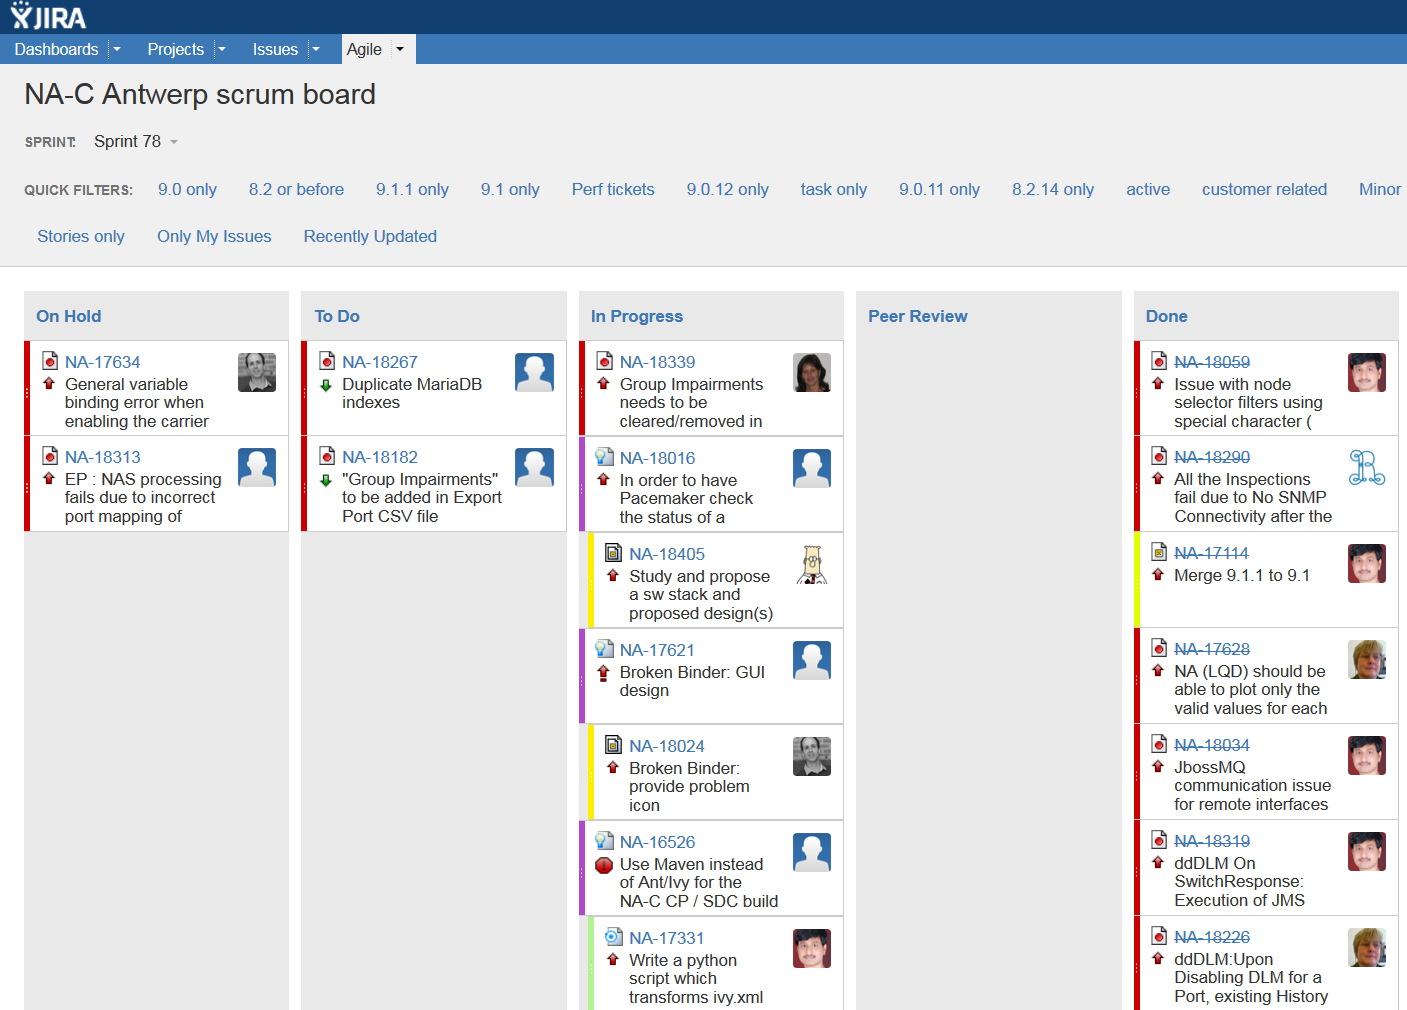
\includegraphics[width=90mm]{CaptureJira.png}
\caption{Het JIRA dashboard van het NA-C team in Antwerpen.} 
\label{jira}
\end{figure}

In het NA-C team heeft men sprints van twee weken, wat wil zeggen dat men elke twee weken een evaluatie doet van het werk dat in de afgelopen twee weken verzet is en welke veranderingen er naar de volgende sprint toe moeten doorgevoerd worden. Aan het begin van een sprint is er dan de sprint planning, waarin er bekeken wordt wat er moet gebeuren met welke prioriteit en wie wat gaat doen, op een heel algemeen niveau. Men maakt hierbij gebruik van user-stories, die een bepaalde taak omschrijven en de subtaken ervan. Het beschrijft wat de gebruiker nodig heeft bij het uitvoeren van zijn taak en bepalen zodus wat er moet ontwikkeld worden om de gebruiker hierbij te helpen. Het omschrijft het "wie", "wat" en "waarom" van deze vereisten op hoog niveau. Een voorbeeld van een user-story is te zien in Figuur \ref{user_story}. Aan het einde van de sprint is er de sprint review, waarbij besproken wordt wat er bereiekt is en waarbij er eventueel demo's gegeven worden van wat er gerealiseerd is. Ook is er de sprint retrospective, waarbij men gaat oplijsten wat er goed en minder goed is gegaan, welke problemen er (binnen het team) waren en hoe deze opgelost kunnen worden.

\begin{figure}[ht!]
\centering
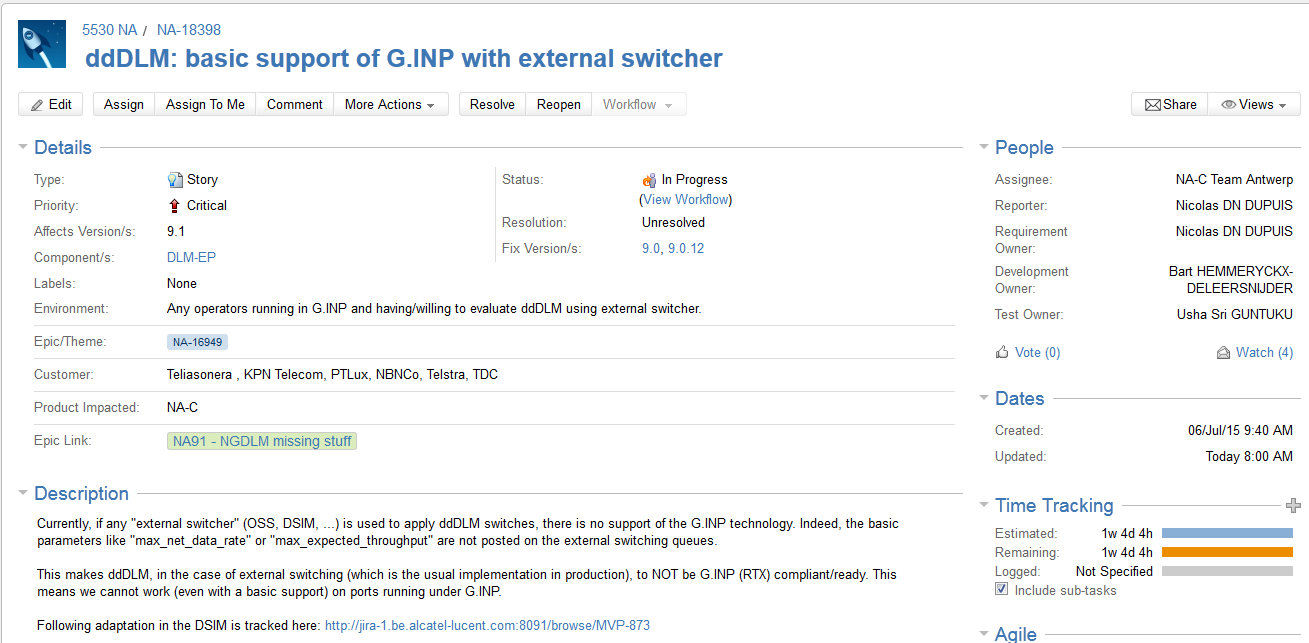
\includegraphics[width=90mm]{user_story.png}
\caption{Een van de user stories van het team van NA-C in Antwerpen.} 
\label{user_story}
\end{figure}

\subsubsection{Continuous integration}
Aangezien er regelmatig releases van software zijn, doet men aan continuous integration, wat inhoudt dat wanneer iemand klaar is met het schrijven van een stuk code en deze commit, alle builds en testen hierrond automatisch zullen runnen zodat fouten in een vroeg stadium kunnen gevonden en opgelost worden.\\
In Antwerpen maakt men gebruik van Jenkins\footnote{https://jenkins-ci.org/}, een open-source continuous integration systeem. Jenkins heeft een dashboard dat een overzicht toont van alle builds, maar je kan ook filteren op zelfgemaakte criteria, zodat je enkel de status van bepaalde builds ziet. Een screenshot van dit dashboard is te zien in Figuur \ref{jenkins}. Het overzicht van elke build toont een gekleurde bol om aan te geven of de laatste build geslaagd (groen/blauw) of gefaald is. Als er testen gefaald zijn, dan zal de bol geel kleuren.
Er is ook een weerbericht dat toont hoe stabiel de build is, waarbij slecht weer duidt op een instabiele build en goed weer op een stabiele build. 

\begin{figure}[ht!]
\centering
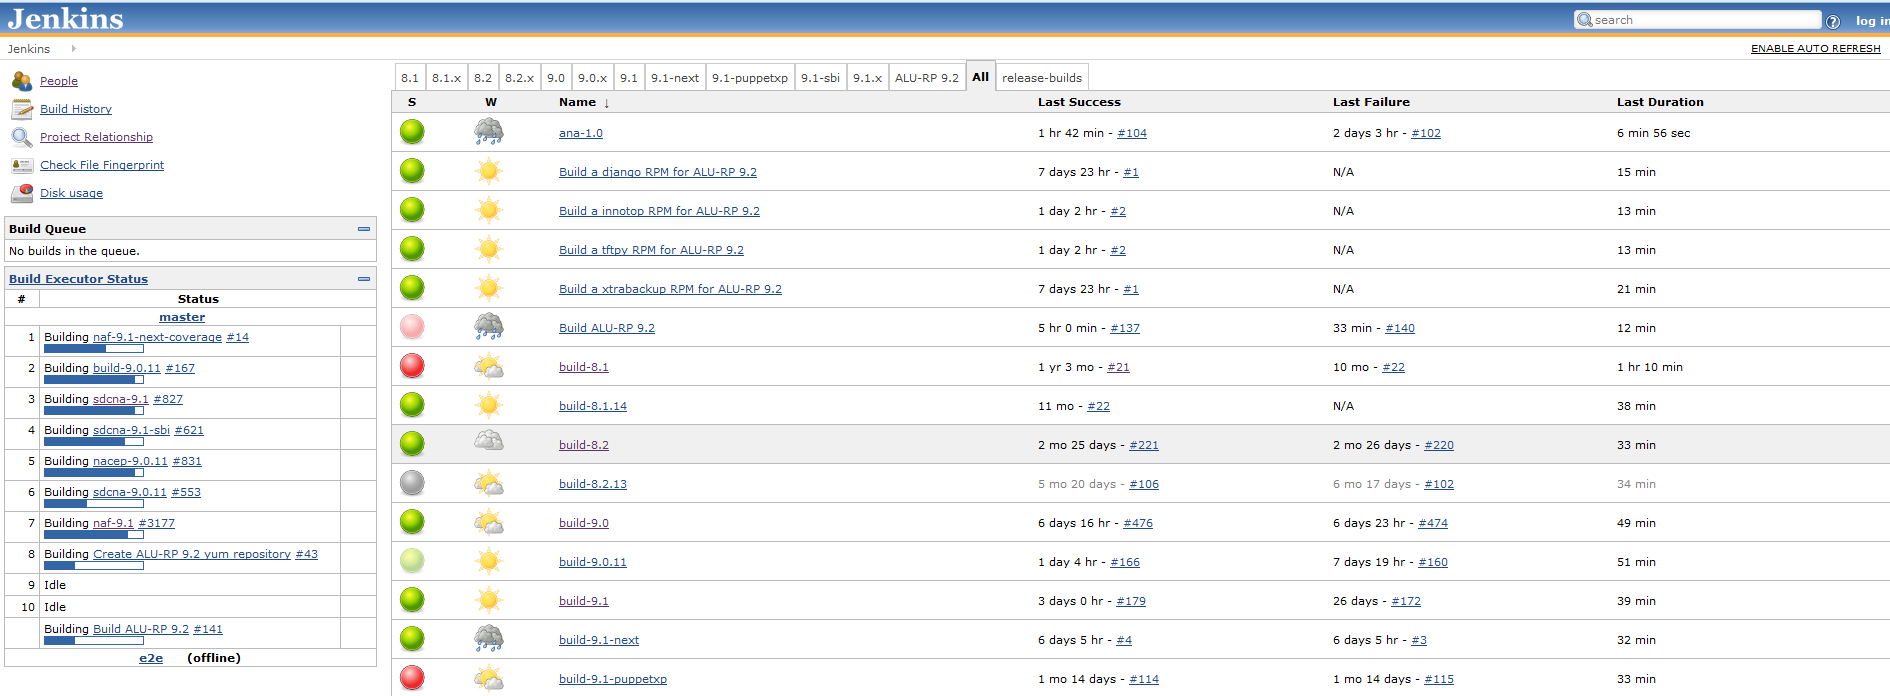
\includegraphics[width=90mm]{CaptureJenkins.png}
\caption{Het Jenkins dashboard, zoals oorspronkelijk gebruikt op de afdeling NA-C in Antwerpen.} 
\label{jenkins}
\end{figure}

Het probleem met dit dashboard is dat het niet echt overzichtelijk is. De kleur van de bollen trekt wel de aandacht, maar als je wil zien over welke build het gaat, is dit niet leesbaar, tenzij je je vlak voor het scherm bevindt. Het Jenkins dashboard wordt op de werkvloer weergegeven op een grote televisie, maar men heeft niet de neiging hiernaar te kijken tijdens de uren, waardoor gefaalde builds enkel maar zichtbaar worden voor het team wanneer ze zelf Jenkins openen op hun PC of tijdens de stand-up meeting. Zoals op Figuur \ref{tv_1} te zien is, moet je zelfs als je voor het dashboard staat goed kijken waar de build staat waarin je ge\"interesseerd bent.

\begin{figure}[ht!]
\centering
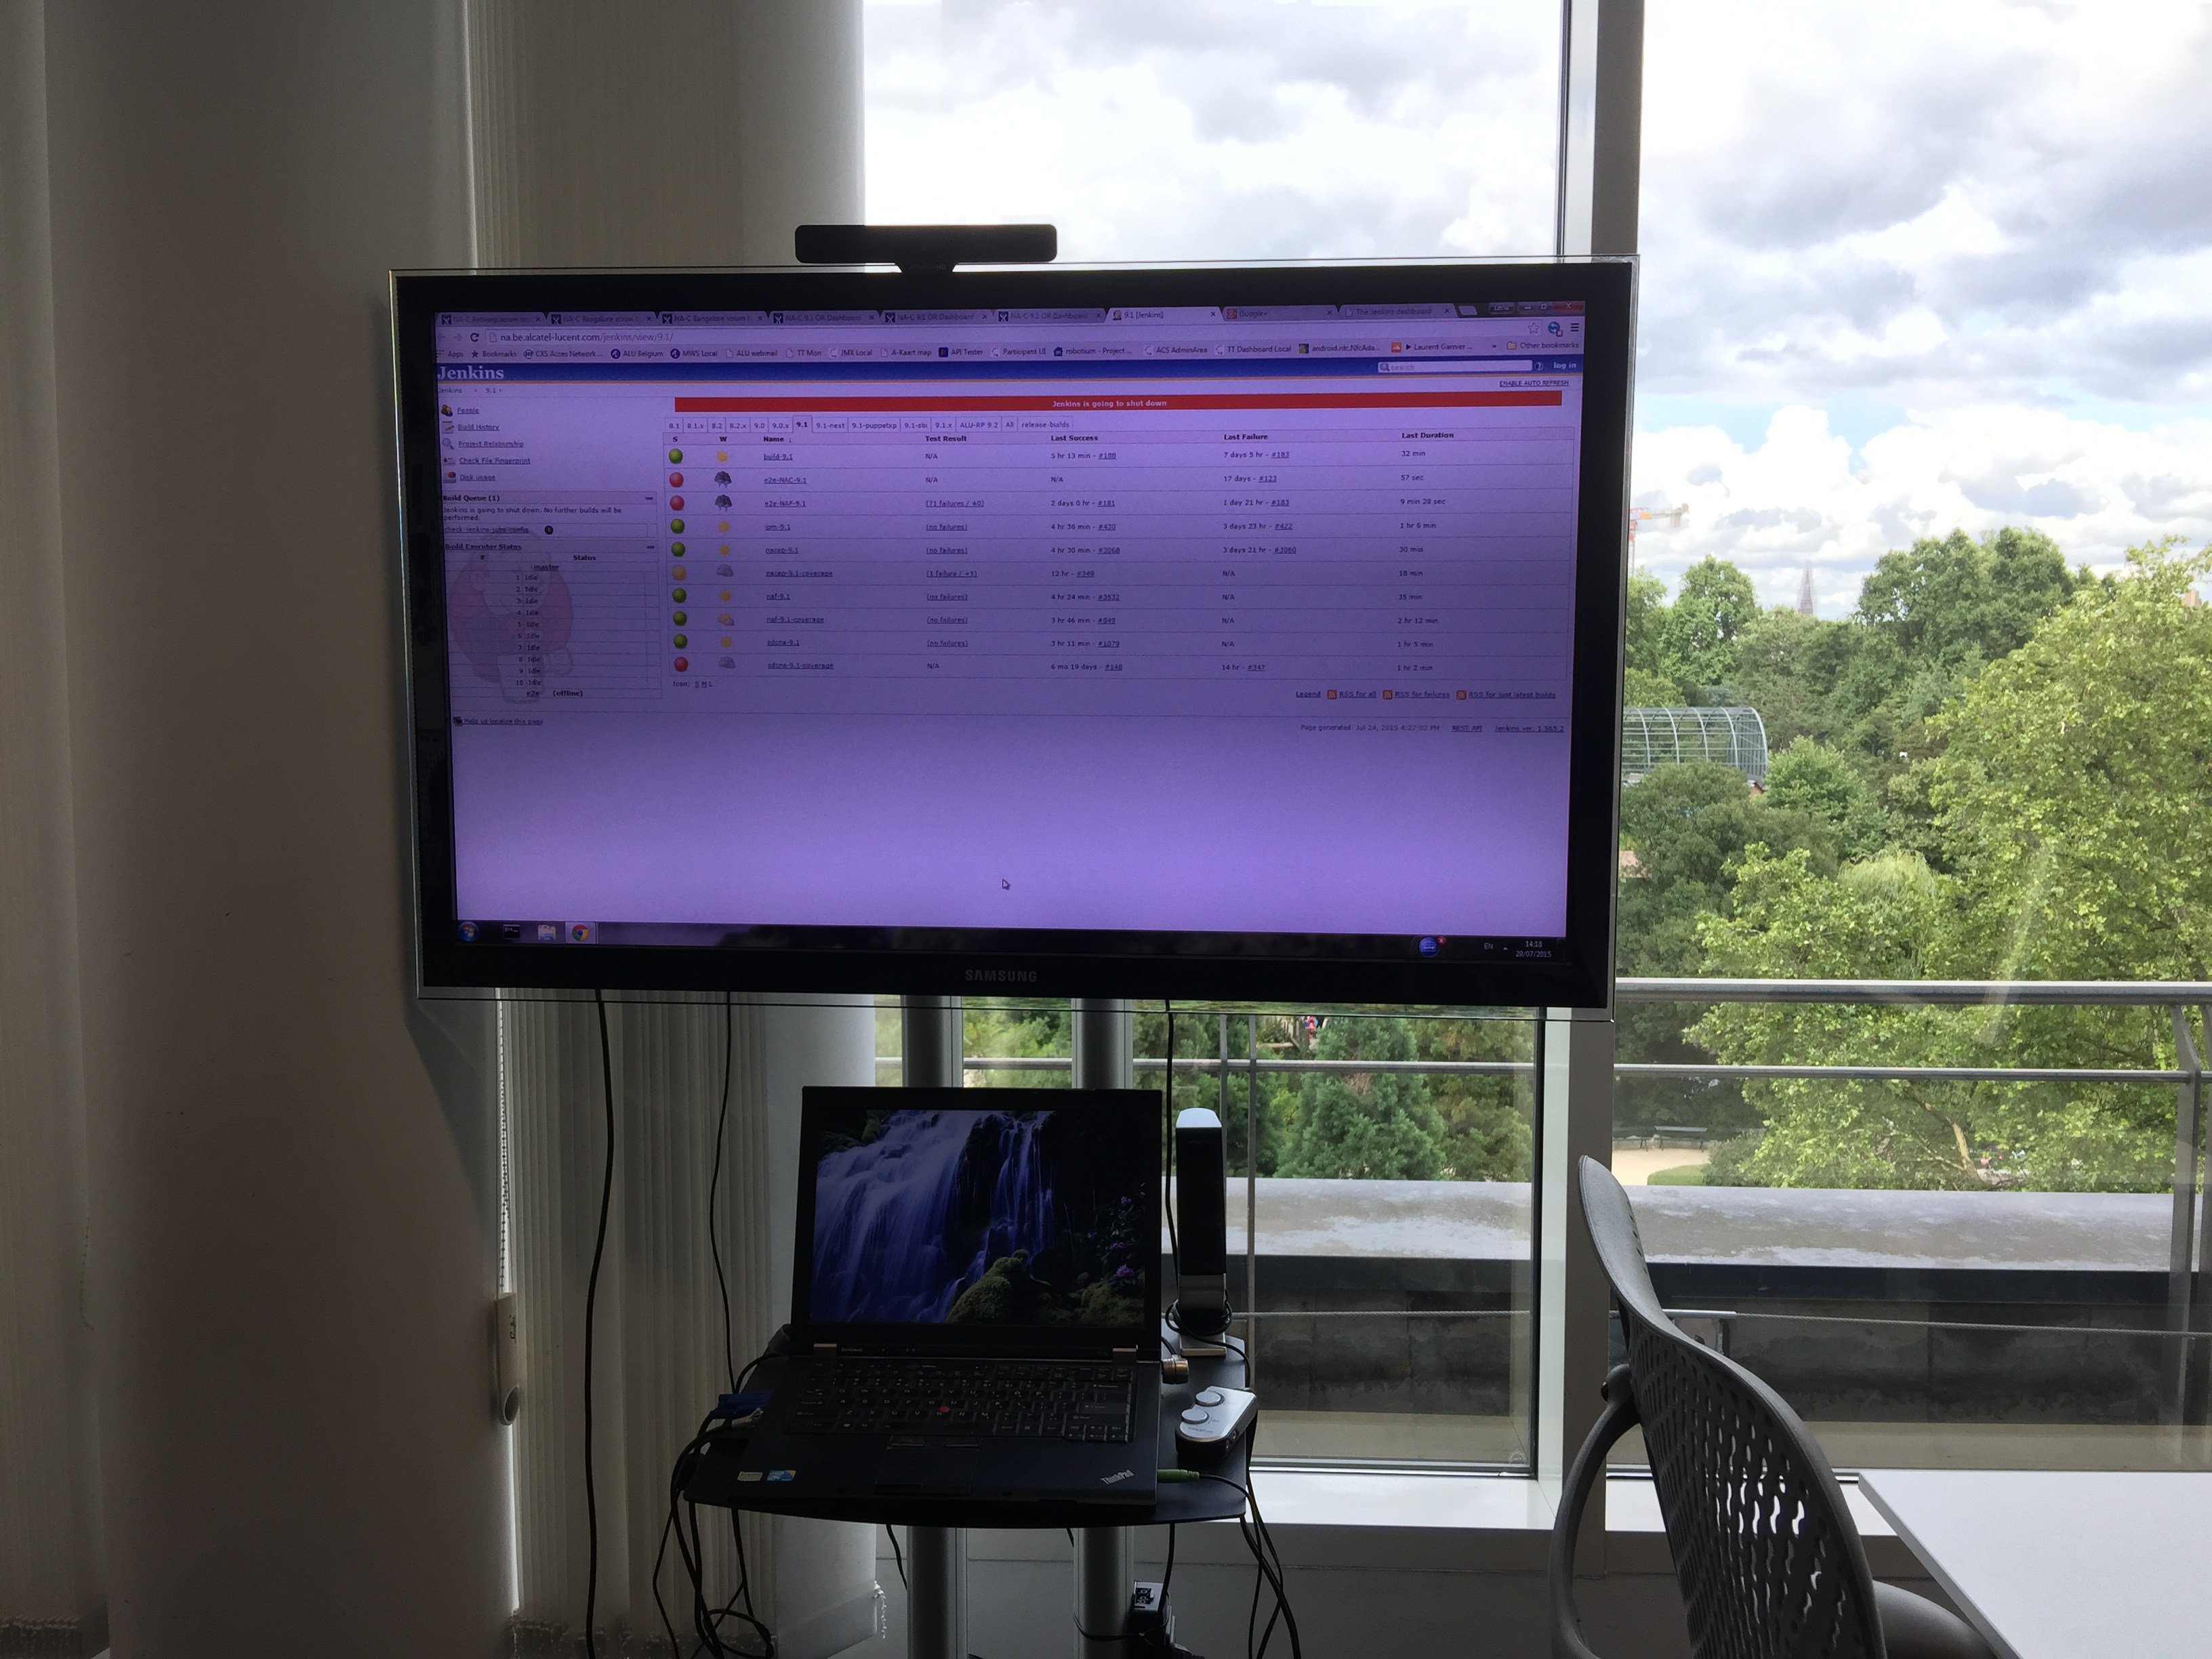
\includegraphics[width=90mm]{tvdashboardoriginal.jpg}
\caption{Het originele Jenkins dashboard weergegeven op de televisie op de afdeling van NA-C in Antwerpen.} 
\label{tv_1}
\end{figure}

\subsection{Stage-opdracht}
\label{opdracht}
Mijn stage-opdracht bestond erin om Jenkins awareness te cre\"eren aan de hand van een dashboard dat een beter overzicht toont.
Als fouten meer in het oog springen, kunnen ze nog sneller verholpen worden en doet men meer aan continuous integration dan wanneer deze fouten pas opgemerkt worden wanneer de programmeur in kwestie zelf het initiatief moet nemen om de resultaten op te zoeken. Gedurende heel mijn stage werd ik enorm betrokken bij alles wat het team deed, zo deed ik dagelijks mee aan de stand-up meetings en werd ik meegevraagd in de sprint planning, sprint review en de retrospective, om zo een idee te krijgen hoe het er in een bedrijf aan toe gaat. Ook al kon ik niet meteen volgen waar ze het over hadden, het heeft me enorm veel bijgeleerd over hoe deze manier van werken het team sterker kan maken gezien iedereen (bijna) dagelijks updates krijgt over wie waarmee bezig is en hoe de korte evaluatieperiodes ervoor zorgen dat er kort op de bal gespeeld kan worden.\\
Er werd voor gezorgd dat ik mijn eigen project kreeg, waarbij er dan ook tweewekelijkse sprints gepland werden, zodat ik zelf kon ervaren hoe deze manier van agile werken in elkaar zit. Er werd voor mij een JIRA-pagina aangemaakt, waarop ik mijn vooruitgang kon bijhouden door taken aan te maken die ik wou doen en problemen kon rapporteren. Een screenshot van mijn JIRA-dashboard is te zien in Figuur \ref{my_jira}.
Mijn eerste sprint bestond uit het maken van een literatuurstudie, te vinden in Appendix \ref{lit_study}, om zo te zien waarop ik moet letten bij het maken van een (goed) dashboard en wat er verbeterd kan worden aan het originele Jenkins dashboard. Eens ik me een idee gevormd had van hoe ik wou dat het dashboard eruit zou zien, heb ik enkele voorstellen opgemaakt en een kleine enqu\^ete gemaakt binnen het team, om te kijken welke voorkeuren zij hadden. Hierop wordt dieper ingegaan in sectie \ref{sprint1}.\\
Vervolgens ben ik begonnen met het implementeren van het dashboard, dit was mijn tweede sprint. Het proces van hoe ik tot het resultaat ben gekomen, is te vinden in sectie \ref{sprint2}.\\
De derde en laatste sprint bestond uit het voorstellen van de eerste versie van het dashboard en hierover feedback krijgen, om het dashboard vervolgens te verbeteren. Tijdens de eindfase van deze sprint werd het dashboard in gebruik genomen op de Jenkins server van Alcatel-Lucent. Dit wordt besproken in sectie \ref{sprint3}.

\begin{figure}[ht!]
\centering
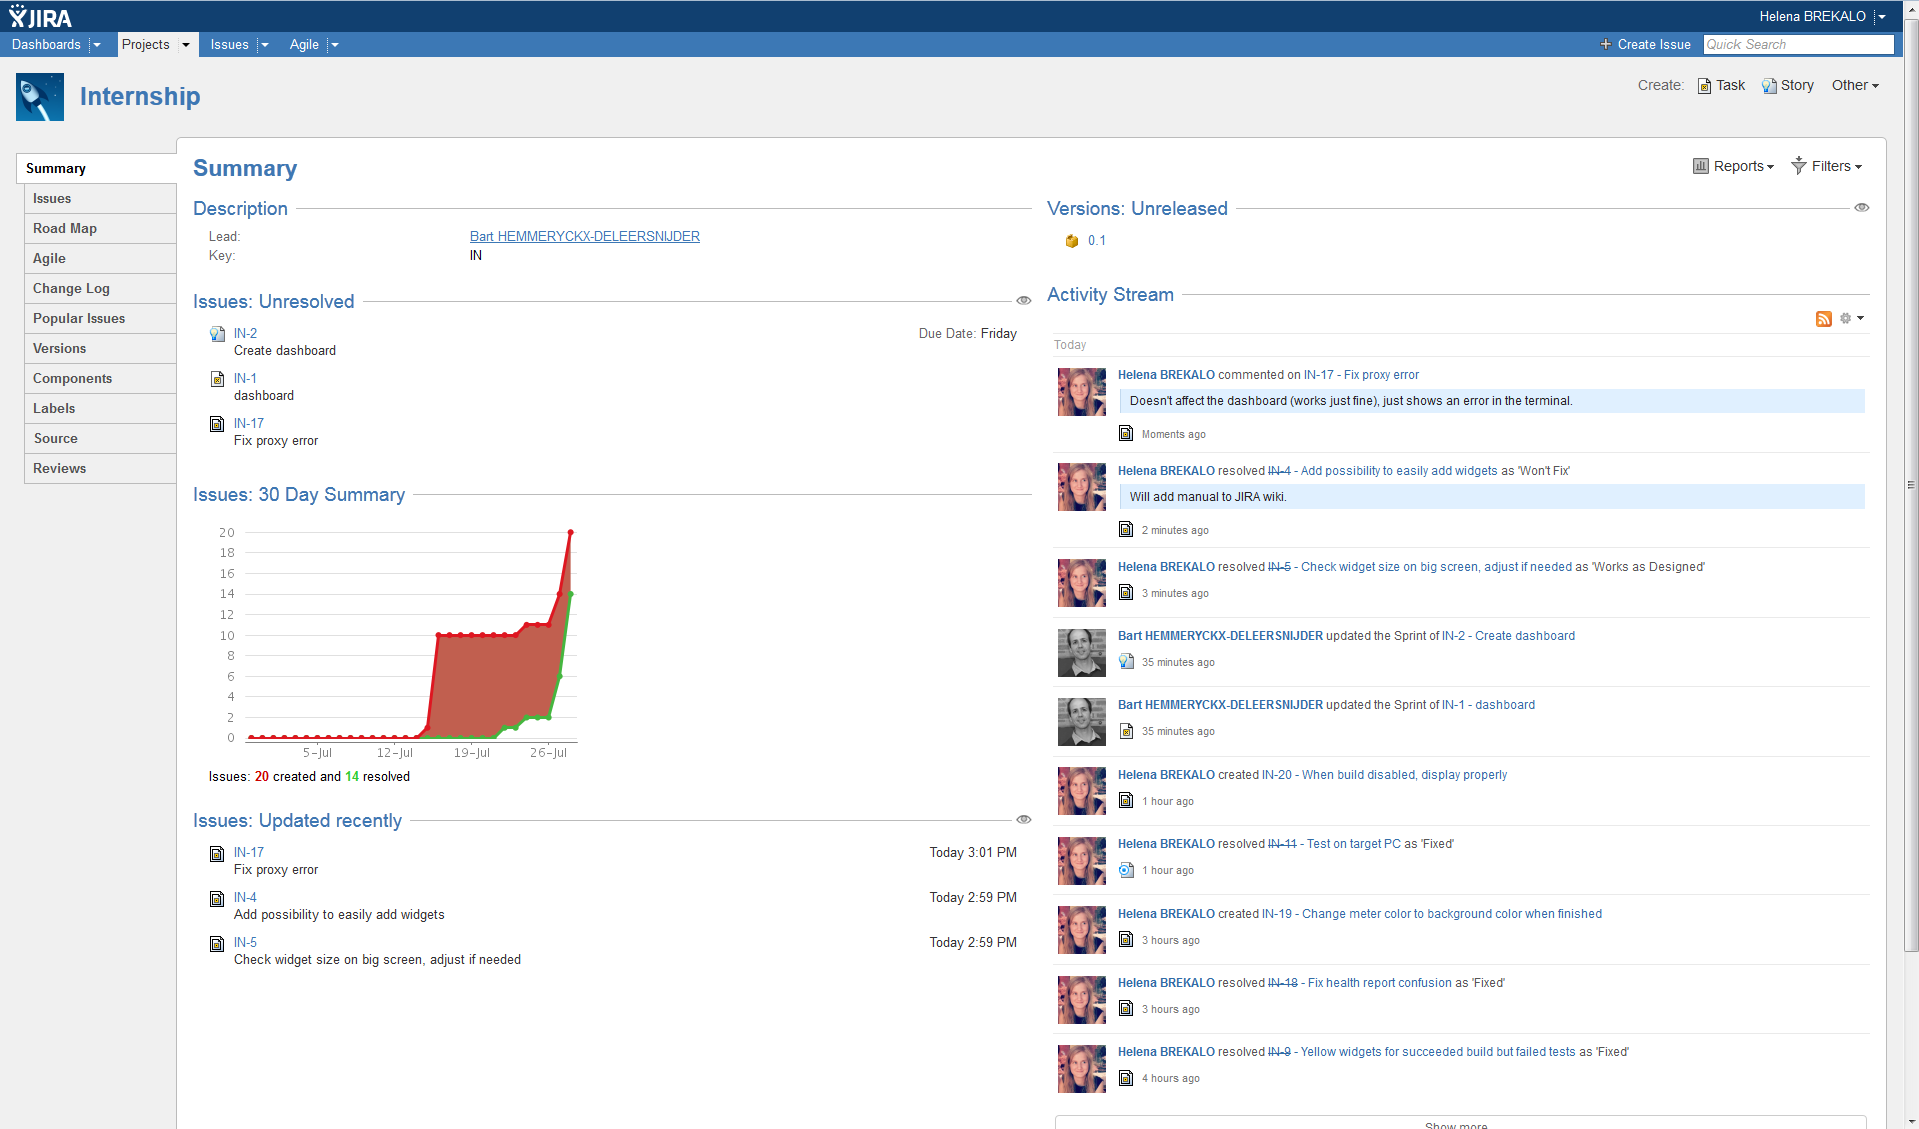
\includegraphics[width=90mm]{myJIRAscreenshot.png}
\caption{Het JIRA-dashboard voor mijn stage.} 
\label{my_jira}
\end{figure}

\subsubsection{Sprint 1: Onderzoek en literatuurstudie} 
\label{sprint1}
\paragraph{Literatuurstudie} Tijdens de eerste sprint heb ik onderzoek gevoerd naar hoe goede dashboards eruit zien en hoe je ze overzichtelijk kan houden. Hierrond heb ik een literatuurstudie gemaakt, die gevonden kan worden in Appendix \ref{lit_study}. Uit deze literatuurstudie bleek inderdaad dat het voorziene Jenkins dashboard niet voldeed aan veel van de vereisten, aangezien je niet in \'e\'en oogopslag de belangrijkste info kan vergaren.\\
Naast de literatuurstudie heb ik ook gezocht naar tools om dashboards te maken, waarbij ik van een collega op de afdeling de aanbeveling kreeg om Dashing\footnote{http://dashing.io/} te gebruiken. Na het bekijken van nog enkele andere tools om dashboards te ontwikkelen, heb ik uiteindelijk voor Dashing gekozen, aangezien het enorm veel flexibiliteit biedt.
\paragraph{Enqu\^ete}
Na het onderzoek en de literatuurstudie, heb ik een voorstel voor dashboardontwerpen gemaakt en deze voorgelegd aan de mensen bij NA-C. Ik liet hen hierbij een kleine enqu\^ete invullen waarbij ze konden kiezen voor verschillende designs en waarbij opmerkingen gegeven konden worden. Uit die opmerkingen zijn nog nuttige commentaren gekomen, waarbij enkele van die idee\"en ook in het dashboard verwerkt zijn. De enqu\^ete en de resultatentabel zijn ook te vinden in Appendix \ref{enquete1}. 
\subsubsection{Sprint 2: Ontwikkeling dashboard} 
\label{sprint2}
Op het einde van de eerste sprint heb ik met Bart een sprint review en retrospective gehouden, om te zien waar ik stond. We hebben deze meeting gecombineerd met de sprint planning, waarbij ik mocht aangeven hoe ik van plan was het dashboard uit te werken en met welke tools. Ik werd hierin heel vrij gelaten, zodat ik zelf kon bepalen wat binnen mijn mogelijkheden lag en wat niet.
\paragraph{Gebruikte tools}
Dashing is een dashboard framework dat geschreven is in Sinatra, een open source software web applicatie geschreven in Ruby. De ontwikkeling gebeurde op Linux, waarbij ik gebruik maakte van Ubuntu 14.04. Op deze PC is dan een lokale Jenkins-omgeving opgezet, zodat het dashboard tijdens de ontwikkeling hiermee getest kon worden. Het schrijven van de code gebeurde in gedit en debuggen werd gedaan via de terminal.\\
De "tegels" op het dashboard worden omschreven als "widgets" waarbij je verschillende soorten widgets kan hebben. Ik heb me toegespitst op \'e\'en widget om informatie over Jenkins te tonen\todo{indien RSS ook: erbij zetten!}. Deze widget kan dan gebruikt worden voor verschillende builds, het is niet de bedoeling om voor elke build een nieuw widget te ontwikkelen (tenzij je verschillende informatie wilt tonen op de verschillende Jenkins-widgets).
\paragraph{Gebruikte talen}
Het schrijven van het dashboard is gebeurd in verschillende talen, hieronder een opsomming welke taal gebruikt werden.
\begin{description}
\item[HTML] HTML wordt gebruikt om te bepalen hoe de inhoud getoond wordt op de widget, dus bijvoorbeeld welk deel als titel zal getoond worden en welke onderdelen als paragrafen weergegeven worden. HTML bepaalt ook waar de elementen op de widget staan. De informatie die getoond wordt, wordt via Batman Bindings\footnote{http://batmanjs.org/} uit de JSON data van de Jenkins server geparset.
\item[(S)CSS] CSS wordt gebruikt om de tekst uit de HTML-file op te maken (grootte van de tekst, stijl, kleur,...), waarbij SCCS (Sassy CSS) ervoor zorgt dat je ook variabelen kan gebruiken, wat niet mogelijk is in standaard CSS. Op deze manier kan je code van een bepaalde opmaak hergebruiken via variabelen. 
\item[Javascript] Javascript werd gebruikt in de Batman Bindings, die ervoor zorgen dat de data die van de website geparset wordt, dynamisch gebruikt kan worden in de HTML-files (via data-bind).\todo{is dit te diep erop ingegaan?} Op zich is de Batman Bindings-library klaar om te gebruiken, maar om een tijdstip te parsen (dat werd weergegeven als Unix timestamp), heb ik nog enkele lijnen Javascript-code moeten toevoegen, alsook de moment.js-library.
\item[Coffeescript] Coffeescript is een taal die transcompileert naar Javascript. De .coffee-file voor een widget specifi\"eert hoe de data, die via de HTML-file opgevraagd wordt, weergegeven wordt. Deze file was van belang om bijvoorbeeld het juiste weerbericht te tonen. Het coffeescript parset de data die via de Batman Bindings werd opgehaald en geeft aan hoe deze doorgegeven wordt aan de HTML-file. Zonder de .coffee-file zou er enkel \textit{plain text} (mits wat opmaak door CSS) te zien zijn op de widget.
\item[Ruby] Dashing maakt gebruik van Embedded Ruby om te bepalen welke tegels getoond worden op het dashboard en van plain Ruby om de data op te halen en te parsen vanuit de juiste plaats (nl. de Jenkins server) via de JSON-data die werd voortgebracht hierdoor. Ook wordt hier de link gelegd tussen de build jobs die getoond \emph{kunnen} (niet per s\'e zullen\footnote{Welke build jobs getoond worden, wordt bepaald door de Embedded Ruby file.}) worden op het dashboard.
\item[JQuery] JQuery wordt gebruikt in de Coffeescript-file om CSS-gewijs klassen of ID's te gebruiken van elementen waarop je een bepaalde actie wil uitvoeren.
\item[JSON] JSON werd gebruikt om de data uit van de Jenkins server te parsen, zodat deze opgevraagd kon worden in de Ruby-file.
\end{description}
Omdat geen van deze talen me helemaal eigen was, heb ik enkele dagen genomen om de basics te leren via Codecademy\footnote{https://www.codecademy.com/}, wat voldoende was om me op weg te zetten.\\
De verschillende bestanden worden als volgt gebruikt:
\begin{itemize}
\item Een widget wordt opgesteld door middel van een .HTML-file, een .scss-file en een .coffee-file.
\item Een Embedded Ruby file geeft via HTML-blocks aan welke build jobs getoond worden op het dashboard.
\item Een plain Ruby file doet de mapping van de JSON data op de variabelen in het dashboard en defini\"eert de namen van de build jobs die getoond kunnen worden.
\end{itemize}
\paragraph{Sprint Review} Op het einde van de tweede sprint werd mij gevraagd om de eerste versie van het dashboard te demonstreren voor het team in Antwerpen, Bangalor en Chennai. Ik kon een werkend dashboard tonen dat informatie toonde over de Jenkins build jobs die op mijn lokale server draaiden. De feedback hierop was positief en enkele vragen van mensen in de verschillende teams konden beantwoord worden. \todo{goed gezegd?}
\subsubsection{Sprint 3: Feedback en verbetering}
\label{sprint3}
Na de sprint review heb ik de Alcatel-Lucent Jenkins-server ge\"integreerd in het dashboard, wat nog anderhalve dag van debugging vroeg, gezien de Jenkins-server nu niet lokaal runde, maar op een andere server. Ook gebruikt men bij Alcatel-Lucent een andere versie van Jenkins, waardoor bepaalde sleutelwoorden waarop geparset wordt anders heten.\\
Na de sprint retrospective van sprint 2 en de sprint planning van sprint 3 heb ik nog een enqu\^ete gedaan om positieve en negatieve puntjes te verzamelen waar men bij de voorstelling van het dashboard tijdens de demo misschien niet was opgekomen. De resultaten van deze enq\^ete zijn te vinden in de appendix.\todo{verwijzing toevoegen}
\paragraph{Ingebruikname} \todo{over vertellen}
\subsection{Resultaat}
\label{resultaat}
De eerste versie van het dashboard is te zien in Figuur \ref{dash_1}. Het dashboard in zijn huidige vorm is gemaakt om getoond te worden op een HD-scherm met 16:9-ratio. Het is de bedoeling dat er zes tegels naast elkaar kunnen staan en dat er drie rijen zijn, wat maakt dat de status van 18 build jobs gelijktijdig getoond kunnen worden. Dit bleek ruim voldoende voor het NA-C team, aangezien er altijd maar op enkele builds tegelijkertijd gefocust wordt.\todo{Indien er een definitieve (dwz veranderde) versie is, praat erover!}

\begin{figure}[ht!]
\centering
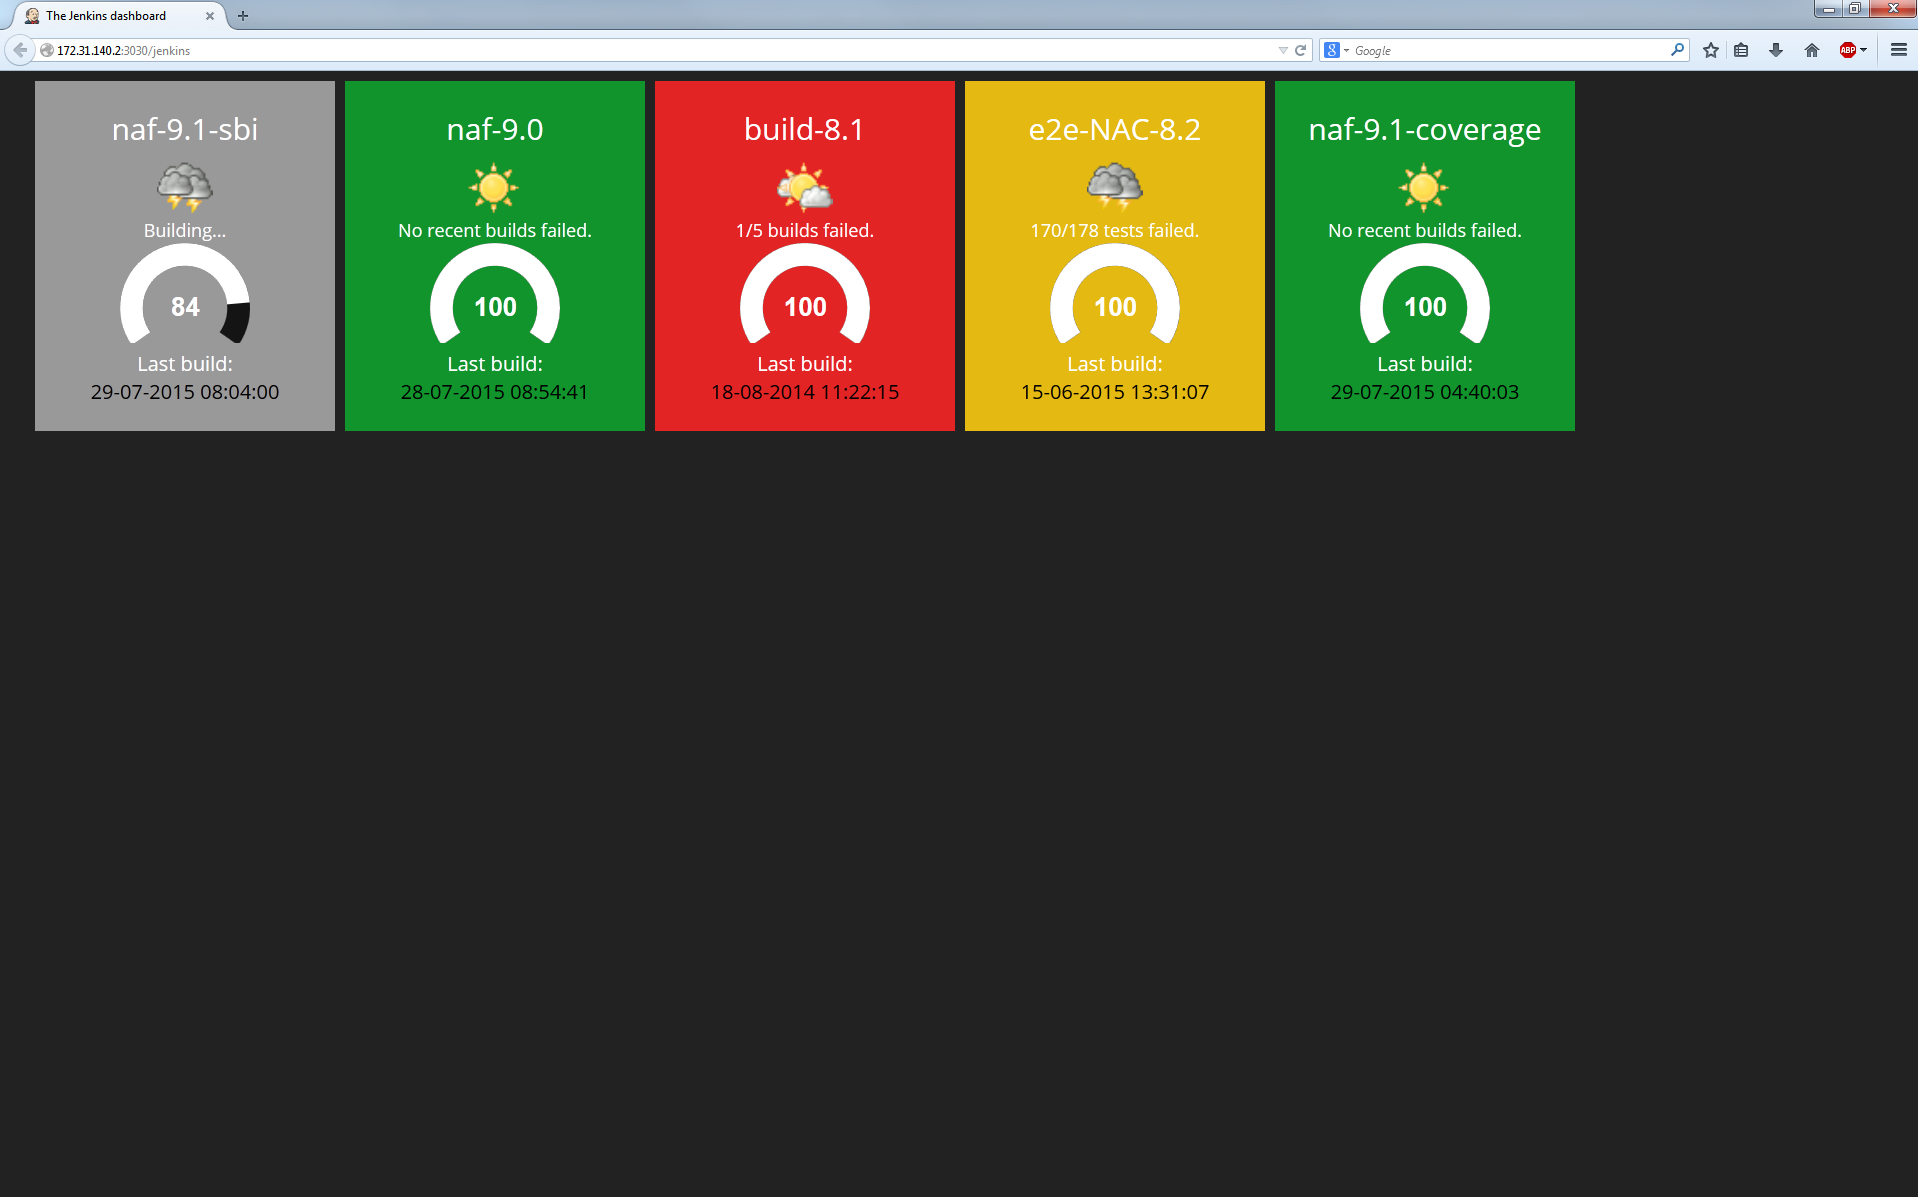
\includegraphics[width=90mm]{dashboard_screenshot1.png}
\caption{Eerste versie van het dashboard.} 
\label{dash_1}
\end{figure}

Figuur \ref{dash_2} toont de tegels in meer detail. De titel is de naam van de build waarover de tegel informatie verschaft. Het weerbericht toont de stabiliteit van de build, of, indien er testen gefaald zijn, de stabiliteit van de testen. De tekst eronder geeft aan hoe stabiel de builds/testen zijn, de meter geeft aan hoe ver de build is in zijn vooruitgang en de timestamp daaronder toont wanneer de laatste build uitgevoerd is.
Er zijn verschillende achtergrondkleuren gebruikt, die de status van de laatste build weergeven:
\begin{itemize}
\item Grijs: de build is nog bezig, het weerbericht toont de stabiliteit van de builds voor degene die nu bezig is.
\item Rood: de laatste build is gefaald.
\item Geel: \'e\'en of meerdere testen zijn gefaald.
\item Groen: de laatste build is geslaagd en alle testen zijn geslaagd. 
\end{itemize}
Als er gekeken wordt naar het voorstel opgemaakt in de literatuurstudie, is de achtergrondkleur daar niet aanwezig (de build status wordt er weergegeven met een gekleurde bol), maar de rondvraag op de afdeling toonde dat iedereen te vinden was voor de gekleurde achtergrond.

\begin{figure}[ht!]
\centering
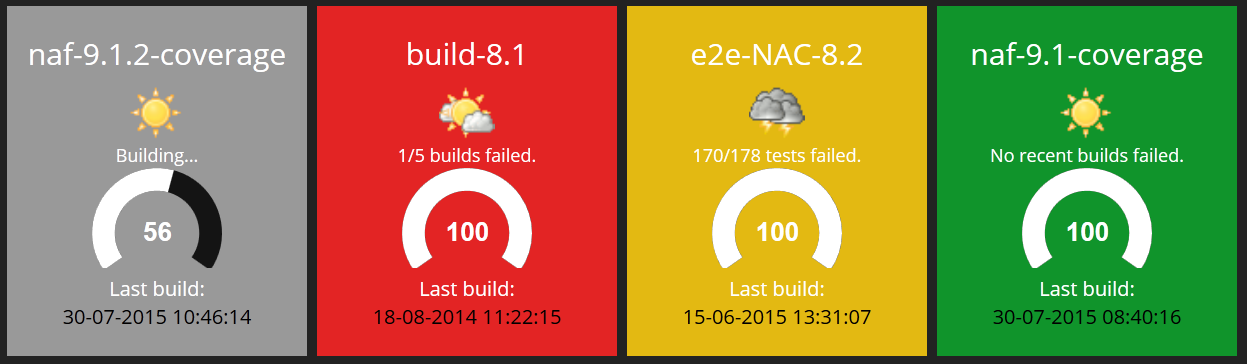
\includegraphics[width=90mm]{screenshot2.png}
\caption{Gedetailleerd overzicht dashboard.} 
\label{dash_2}
\end{figure}

\subsection{Initiatieven voor interns}
\label{interns}
Alcatel-Lucent organiseerde deze zomer een initiatief om alle interns met elkaar in contact te brengen tijdens speciale info-events en meetings. Op deze manier konden interns van verschillende afdelingen met elkaar bespreken hoe de stage op hun afdeling verliep en zo ervaringen met elkaar uitwisselen. Er zijn verschillende contactmomenten georganiseerd, meestal tijdens de middagpauze. Er waren verschillende bijeenkomsten, waaronder samen lunchen om kennis te maken, een gesprek met Joeri Veldeman, begonnen als doctor in de \textit{electrical engineering} bij Alcatel en nu hoofd van de afdeling van human resources. Zijn ongewone carri\`erepad werd ons uitgelegd en hij heeft informeel met ons gepraat over ons verdere studietrajecten.
Verder is er ook een infosessie geweest over ALU Labs, waarin enkele van de zaken aan bod kwamen waarin Alcatel-Lucent investeert en research bij uitvoert.\\
Dit alles maakte dat de stage niet alleen een verrijking van mijn kennis binnen de afdeling werd, maar ook daarbuiten, waarbij contact met andere studenten gelegd werd.

\section{Relatie stage en opleiding}
\label{relatie}
Het doel van de stage was om een dashboard te maken zodat de build status van de verschillende onderdelen van projecten overzichtelijk getoond konden worden. Binnen deze stage werd ik bovendien ook betrokken bij alle bijeenkomsten met het team, om zo te ervaren hoe het er in een werkomgeving aan toe gaat. Op deze manier heb ik extra facetten gezien die tijdens de opleiding aan bod zijn gekomen, die ik niet had gezien moest ik niet zo betrokken geweest zijn bij alles. Zo werkt men hier volgens de agile-methode scrum, met elke dag standup meetings en tweewekelijkse sprints. Dit is iets dat in de lessen van Software-Ontwerp kort aan bod was gekomen, waarvan ik tijdens de stage zag dat het echt zijn nut heeft. De korte sprints en regelmatige reviews zorgen ervoor dat problemen niet te lang kunnen blijven bestaan en omdat er bijna dagelijks gepraat wordt over wie waarmee bezig is, kunnen mensen elkaar vlot helpen en weet iedereen wie waaarmee bezig is. Doordat men gebruik maakt van continuous integration zijn (merge)fouten snel opgespoord en opgelost. Zelf kreeg ik ook eigen scrumproject, waardoor ik ook met sprints werkte en zo "kleine" doelen voor ogen had. Deze manier van werken is vergelijkbaar met die tijdens de P\&O-sessies tijdens de bachelorproef, waarbij we om de paar weken een bepaalde functionaliteit moesten kunnen demonstreren. Op de afdeling NA-C doet men ook regelmatig aan pair-programming, iets wat ook aangeraden was in de sessies van Software-Ontwerp. Aangezien ik aan een eigen project moest werken, heb ik dit niet zo vaak gedaan, maar als ik met vragen zat, kwamen collega's met plezier samen met mij zoeken naar de oplossing en me uitleg geven.\\
Het dashboard dat ik moest maken moest niet een kant-en-klaar dashboard zijn waar ik dan zelf info aan toevoegde, maar \'e\'en waarbij ik zelf moest nadenken over het design en de implementatie van de code om het dashboard te realiseren. Dit werd behandeld in de lessen van Software-Ontwerp.\\
Ik maakte gebruik van een bestaand framework, maar heb zelf nog heel veel van de code moeten schrijven. Dit heeft me er meer dan eens attent op gemaakt hoe belangrijk goede documentatie is, gezien de bestaande code op zich nauwelijks/niet gedocumenteerd was en ik soms moeite had om te begrijpen wat een bepaalde functie deed. Het schrijven van (goede) documentatie is iets waar tijdens de lessen van Objectgericht Programmeren altijd op gehamerd is. De documentatie op de websites van het framework en de plugins  was vaak ook erg kort door de bocht of onvolledig, dus ik heb vaak lang gezocht naar bepaalde zaken. Omdat ik het zelf zo erg miste, heb ik zelf documentatie geschreven, in de hoop dat het voor een eventuele opvolger makkelijker is om alles te begrijpen.\\
Binnen de opleiding wordt er altijd gewerkt in kleine groepjes, meestal van twee mensen, maximaal in groepen van zes mensen. Op de afdeling NA-C werkt men in een team van ongeveer 10 mensen, wat het managen van het team nog moeilijker maakt dan bij een groep van slechts enkele mensen. Toch is er getoond dat dit perfect mogelijk is indien je de juiste tools gebruikt (bij NA-C maakt men gebruik van Confluence en JIRA) en indien er genoeg gecommuniceerd wordt.\\
Tijdens de lessen van Informatica werktuigen zijn Ruby, Linux en LaTeX aan bod gekomen. Ruby bleek nuttig om de (Embedded) Ruby voor het dashboard te schrijven, waar de kennis van Linux ervoor zorgde dat ik iets vlotter mijn weg vond bij het installeren van programma's en het werken met Linux in het algemeen, gezien het dashboard in Linux is ontwikkeld. LaTeX is gebruikt om de literatuurstudie te maken en het verslag op te stellen.\\
Doordat er in de bachelor informatica al een heel aantal programmeertalen gezien werden, was het aanleren van andere (opmaak)talen veel makkelijker. \\
Het schrijven van (wetenschappelijke) verslagen was een groot onderdeel tijdens Wetenschapscommunicatie en tijdens P\&O, wat me hielp bij het schrijven van de literatuurstudie en het stageverslag.\\
Waar versiecontrole tijdens het project van Software-Ontwerp aangeraden, maar niet verplicht was, werd het bij P\&O wel verplicht. Doordat ik hiermee had kennis gemaakt, heb ik hiervan gebruik kunnen maken (zij het aan de late kant, zie de kritische reflectie van de competenties in Sectie \ref{reflectie}) tijdens een groot deel van de stage. \todo{evt. tekst bijvoegen}

\section{Krititsche reflectie competenties}
\label{reflectie}
\begin{itemize}
\item Technische competenties die ik hoopte te verbeteren:
\begin{description}
\item[Bijleren over version control] Er wordt op de afdeling NA-C gewerkt met Git, waar ik ook tijdens mijn opleiding al mee in aanraking ben gekomen. Tijdens de ontwikkeling van het dashboard heb ik geen gebruik gemaakt van Git, hoewel dit zeker nuttig geweest zou zijn bij het schrijven van mijn dashboard. Eens de eerste versie van het dashboard klaar was, is het wel op Git gezet\footnote{De code is te vinden op https://github.com/HelenaCat/jenkins-dashboard}, maar dit had dus veel eerder moeten gebeuren. Er is gebruik van gemaakt bij het toevoegen van documentatie en bij het maken van veranderingen tijdens de derde sprint.\\
Ondanks het te laat beginnen gebruiken van version control, zijn mijn competenties hierrond wel verbeterd, gezien ik Git nu ook via de Linux command line heb leren gebruiken en niet alleen in de grafische user interface op Windows. \todo{dit beter vertellen?}
\item[Leren werken met Jenkins] Op de afdeling NA-C werkt men met het continuous integration systeem Jenkins, dat builds automatisch runt nadat er een nieuwe versie van de software gecommit is. Tijdens de stage was het duidelijk hoe nuttig dit is: er werd op een gegeven moment een fout gemaakt, die ook nog eens onvoldoende getest bleek, maar men heeft deze heel snel ontdekt en binnen de 2 dagen kunnen oplossen. Moest er gewacht zijn met mergen tot vlak voor de release, was men waarschijnlijk veel meer problemen tegengekomen. Continuous integration is vooral handig in teams met meerdere mensen, het was dus van pas gekomen tijdens P\&O of Software-Ontwerp. \todo{dat laatste weglaten?}
\item[Mij inwerken in een reeds lopend project] Ik moest niet meewerken aan de code van het NA-C team zelf, maar heb mij wel moeten inwerken in de code van het dashboard. Zoals hierboven vermeld, was dit niet altijd makkelijk, maar het heeft er wel voor gezorgd dat ik enorm veel heb bijgeleerd, net omdat ik heel veel zelf moest uitzoeken. Eens de eerste versie van het dashboard klaar was, kende ik de code enorm goed, dus nieuwe veranderingen waren zeer snel ge\"implementeerd.
\end{description}
\item Persoonlijke competenties die ik hoopte te verbeteren:
\begin{description}
\item[Leren werken in grote teams] In het NA-C team in Antwerpen werken er een tiental mensen, in Bangalor en Chennai zijn er teams van gelijkaardige grootte. Doordat er dagelijks een standup meeting was met de mensen van het team in Antwerpen, was iedereen goed op de hoogte van wie wat deed en doordat men met sprints van twee weken werkte, kwamen problemen snel boven. Dit is iets dat ik zeker meeneem naar projecten in de toekomst toe, ik heb ervaren hoe al deze zaken kunnen helpen in het beter doen verlopen van een project.
\item[Plannen op lange termijn] Aan het begin van mijn stage werd me meteen gezegd dat ik redelijk vrij gelaten ging worden in mijn planning, maar er werd wel gevraagd om er een op te stellen, zodat ik ook in sprints kon werken. Ik heb zelf voorstellen mogen doen en aan mijn eigen tempo (maar toch binnen de termijnen van de sprints) kunnen werken. Als er grote dingen te doen stonden, plande ik daar altijd genoeg tijd voor in, zodat ik uiteindelijk "te vroeg" klaar was en aan verbeteringen kon werken. Dit is een van de competenties die ik zowel in het tweede semester van mijn laatste bachelorjaar heb aangescherpt, als nu op de stage.  
\end{description}
\end{itemize}

\section{Besluit}
\label{besluit}
Mijn stage ging voor 6 weken door bij Alcatel-Lucent in Antwerpen. Er werd mij gevraagd een dashboard te ontwerpen om de build status van het continuous integration systeem Jenkins te tonen.\\
Het dashboard is succesvol gemaakt binnen de opgelegde tijd met behulp van Dashing, draaiende op een Linux server.\\
Tijdens de stage heb ik enkele (opmaak)talen bijgeleerd, waaronder Javascript, JQuery, HTML en (S)CSS. Mijn kennis van Ruby kwam hierbij ook van pas.\\
Onder de goede begeleiding van Bart heb ik grotendeels zelfstandig mijn doelen en het project uitgewerkt en geleerd hoe het er in een bedrijf aan toe gaat.

\clearpage



\begin{appendices}
\section{Literatuurstudie}
\label{lit_study}


\paragraph{General}
A dashboard is a tool to quickly show information at a glance. Its purpose is to have the "reader" gather information without having to look things up; everything should be clear by having a quick look at the dashboard. At Alcatel-Lucent, they make use of the Jenkins dashboard, but it doesn't comply with the given description: in order to see what builds failed/succeeded, you need to find the build you're looking for and then check its status. It is clear from the -lack of- its use that this way of displaying the information does not suffice, since the TV dashboard is not/barely used but every employer looks up the dashboard on their own PC every once in a while. \\

The purpose of this literature study is to create Jenkins awareness, so the developers can take a look at the TV dashboard a few times a day and have them see how the project is proceeding.\\
One of the most important things is that the information displayed on the dashboard can be easily interpreted. This means that you don't want a cluttered dashboard with too much information so it becomes unclear.
Stephen Few has written an excellent article on the topic, with the main conclusions being:
\begin{itemize}
\item don't show too much information,
\item keep the information simple,
\item colors should be used sparingly or they will mean nothing at all,
\item visuals should be useful; not overwhelming or distracting and
\item the information represented should be accurate, so you should make sure the information is displayed correctly and with enough context.
\end{itemize}
 
This last remark is also made by Matthew Skelton\footnote{http://blog.matthewskelton.net/2013/03/11/what-makes-an-effective-build-and-deployment-radiator-screen/}, who shows that if you only show the failed builds, people will start to ignore the 'alarm signals' the dashboard displays and perform less well compared to when a context is shown, also showing the successful builds. \\
Few’s theory is backed up by the people at Geckoboard, who have made a blog consisting of 6 parts, referencing to Few, but also adding some rules of thumb\footnote{https://www.geckoboard.com/blog/building-great-dashboards-6-golden-rules-to-successful-dashboard-design/}. Every article listed in the appendix refers to Few’s article and some make additional remarks. 
One of them is that it’s very important to keep your audience in mind, the board of directors will want to see different metrics represented in the dashboard than, say, the people of human resources. 
In the case of software developers, they’ll want to see metrics about the build status of the different jobs. Related to this is that not every dashboard will need the same layout and look. \\
In the case of the Jenkins dashboard, charts won’t tell you much, since it doesn’t really tell anything about the status of the last build. Below, the example of the Jenkins dashboard is further explained and a proposal is made that conforms to the guidelines of a good dashboard.

\paragraph{Improving the Jenkins dashboard}
The Jenkins dashboard, as seen in Figure \ref{jenkins}, displays a list of the builds of a project, together with a colored dot and a "weather report". The dot displays information about the last build, the color indicating whether it failed or succeeded and a flashing dot meaning the build is still in progress. 
The color of the dot at that time then refers to the last finished build.
The weather report tells you something about the stability of the builds. If the weather looks good, then the build is stable. The worse the weather gets, the less stable the build is. This way, you get an overall view about the stability of the different build jobs.

\begin{figure}[ht!]
\centering
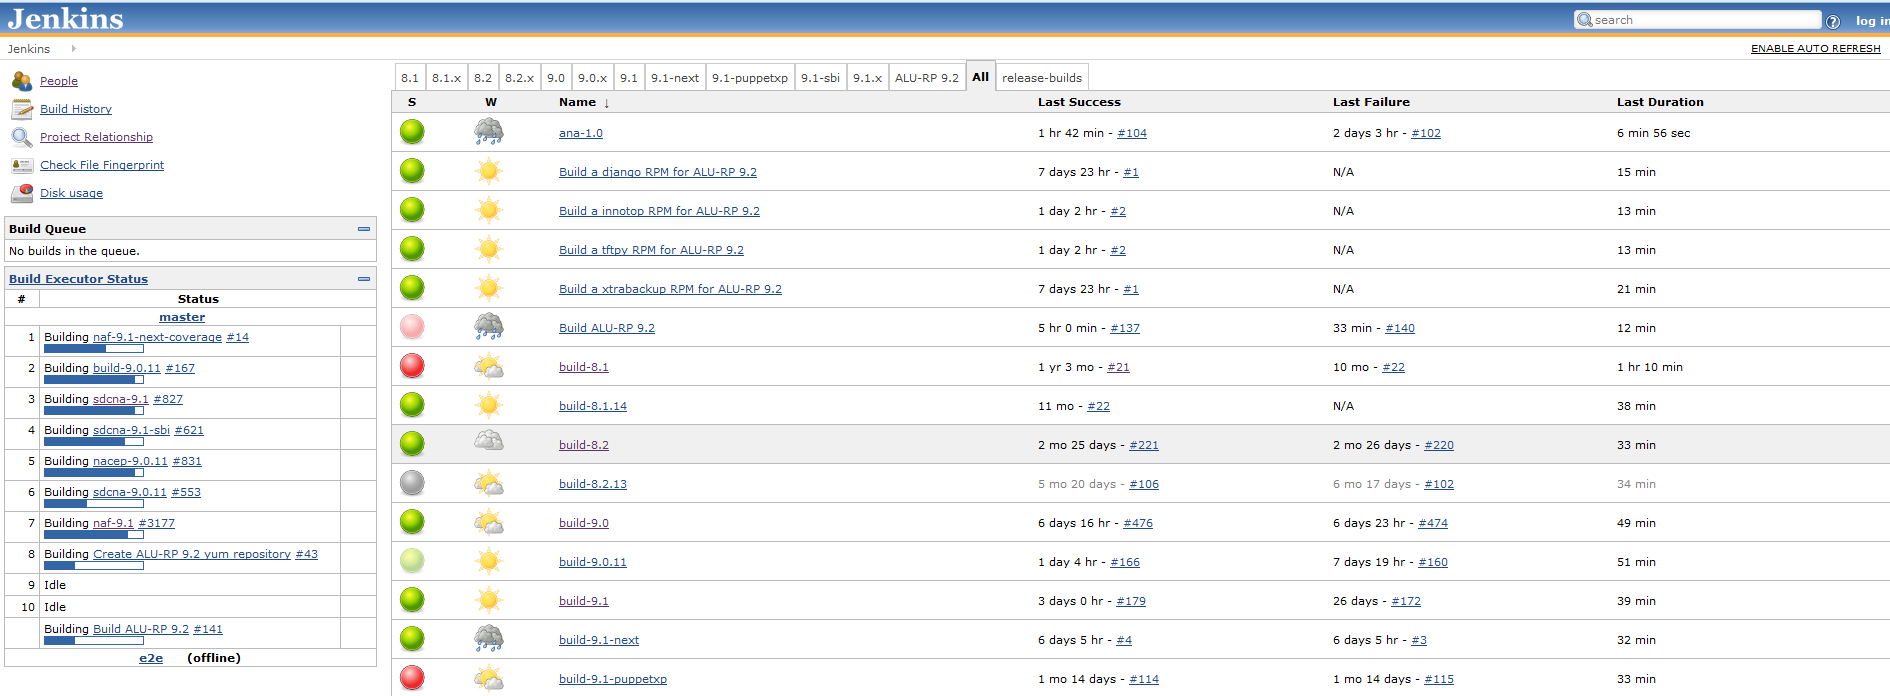
\includegraphics[width=90mm]{CaptureJenkins.png}
\caption{The Jenkins dashboard.} 
\label{jenkins}
\end{figure}
 
These two things give you a fairly good overview, but the downside of the dashboard is that you have to be right in front of the screen to see what job the colored dot and the weather report are referring to. 
The details of the build job are in plain text, so if you want to project it on a TV screen, people will have a hard time knowing what builds are doing well and which ones aren't.
There are plug-ins available that show a dashboard, but they none of them comply with the most important rules described above: they're either too crowded or use too much color, distracting the viewer from what's really important.

\begin{figure}
\centering
\begin{minipage}{0.45\textwidth}
\centering
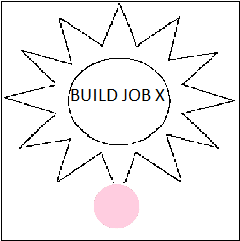
\includegraphics[width=60mm]{prop1.png}
\caption{Proposal 1.}
\label{prop1}
\end{minipage}\hfill
\begin{minipage}{0.45\textwidth}
\centering
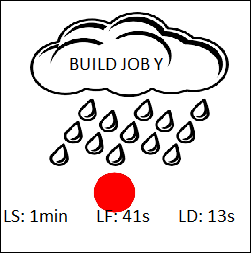
\includegraphics[width=60mm]{prop2.png}
\caption{Proposal 2.}
\label{prop2}
\end{minipage}
\end{figure}
  
The proposed images, as seen in Figure \ref{prop1} and \ref{prop2} comply with the design problems to be avoided as proposed by Stephen Few:
\begin{itemize}
\item Too much complexity
\item Too many alert conditions
\item Alerts that cannot be differentiated
\item Overwhelming visuals
\item Distracting visuals
\item Inappropriate visual salience
\item Mismatch between information and its visual representation
\item Indirect expression of measures
\item Not enough context
\end{itemize}
The images show the build stability together with the success or failure of the last build and show the name of the build clearly. It's also possible to add a timestamp of when the last success and failure were and the last duration at the bottom of the tiles, as shown in Figure \ref{prop2}. If you have color blind people in your team (as Few pointed out might happen), you could replace the green dot by a very light red dot, indicating it doesn't need attention, as shown in Figure \ref{prop1}.
This could be realized using existing Jenkins plug-ins and changing them. The Radiator View\footnote{http://blog.matthewskelton.net/2013/03/11/what-makes-an-effective-build-and-deployment-radiator-screen/} seems like a good basis.
An alternative could be to implement already existing software like Dashing\footnote{dashing.io}, which provides the tools to generate dashboards very easily. Instead of showing the weather as proposed, color codes may be used for the tile backgrounds, either representing the status of the last build or the status of the past builds. A combination is also possible where the color represents the status of the last build and an opaque weather report image as the background. An example is given in Figure \ref{dash}:

\begin{figure}[ht!]
\centering
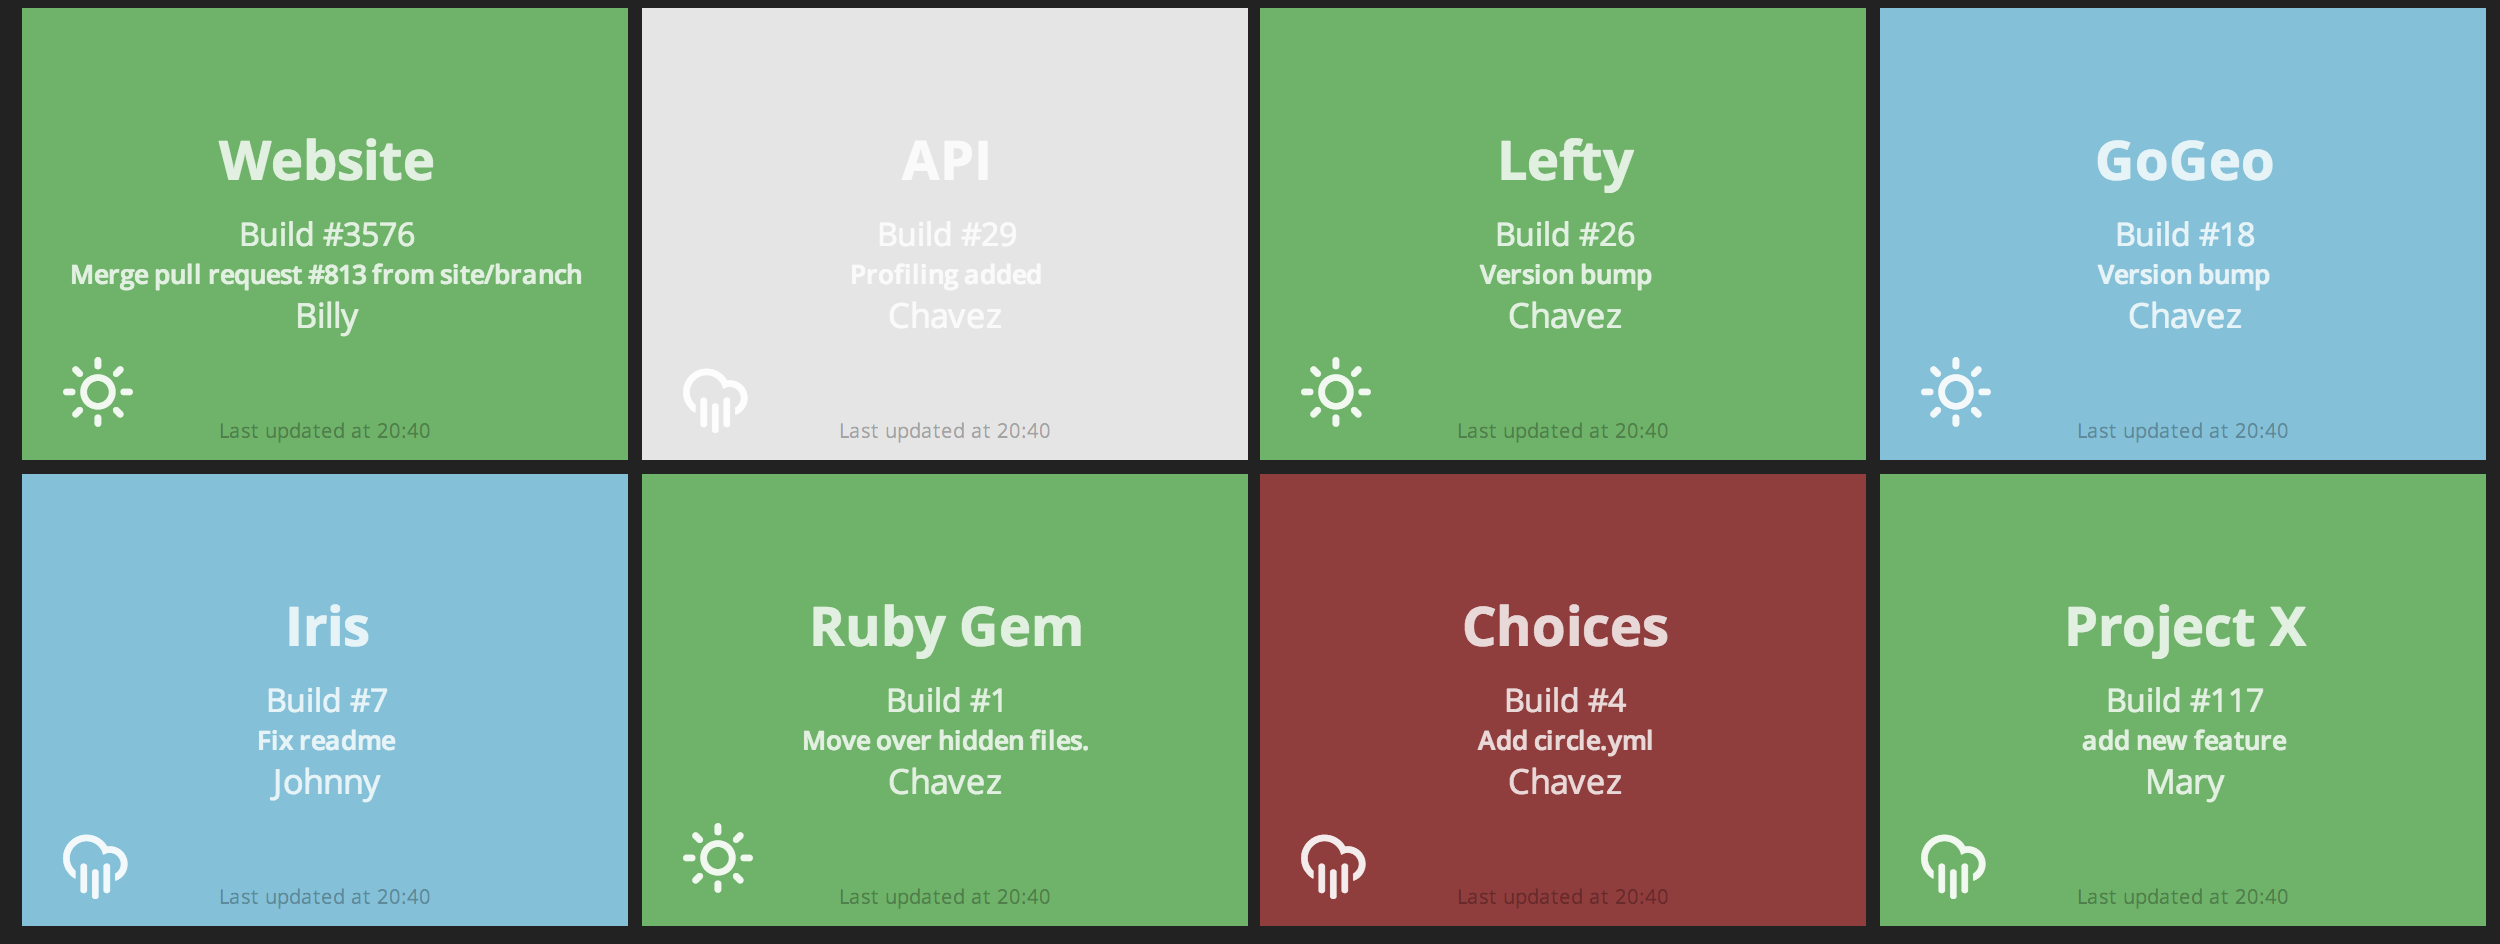
\includegraphics[width=90mm]{dashboard-prop.png}
\caption{Example dashboard for Jenkins.} 
\label{dash}
\end{figure} 
 
The colors aren’t too overwhelming and they’re meaningful, since people are used to the colored dots in the Jenkins dashboard. 
A third, less tile-oriented dashboard is Team Dashboard\footnote{http://fdietz.github.io/team\_dashboard/}. It also supports Jenkins plug-ins.


\begin{thebibliography}{11} 

\bibitem{few} Stephen Few, \emph{Dashboard Design For Real-Time Situation Awareness}, http://www.perceptualedge.com/articles/Whitepapers/Dashboard\_Design.pdf, consulted on 09/07/2015

\bibitem{skelton} Matthew Skelton, \emph{What Makes an Effective Build and Deployment Radiator Screen?}, http://blog.matthewskelton.net/2013/03/11/what-makes-an-effective-build-and-deployment-radiator-screen/, consulted on 09/07/2015

\bibitem{smith} Nick Smith, \emph{Designing and Building Great Dashboards - 6 Golden Rules to Successful Dashboard Design}, https://www.geckoboard.com/blog/building-great-dashboards-6-golden-rules-to-successful-dashboard-design/, consulted on 09/07/2015

\bibitem{gemignani} Zach Gemignani, \emph{A Dashboard Alerts Checklist}, http://www.juiceanalytics.com/writing/dashboard-alerts-checklist/, consulted on 09/07/2015

\bibitem{juice} No author specified, \emph{A Guide to Creating Dashboards People Love to Use}, http://www.cpoc.org/assets/Data/guide\_to\_dashboard\_design1.pdf, consulted on 10/07/2015

Images:

\bibitem{sun} \emph{Sun}, http://azcoloring.com/coloring-page/112445

\bibitem{rain} \emph{Rain cloud}, http://www.clipartpanda.com/categories/animated-rain-clouds

\bibitem{red_dot} \emph{Red dot}, http://www.thepointless.com/reddot

\bibitem{pink_dot} \emph{Pink dot}, http://www.create-a-mural.com/dry-erase-11-soft-pink-dot-decal.html

\bibitem{dashboard} \emph{Example dashboard},  https://camo.githubusercontent.com/
1509a366bd27fad24ba09c45793308a85bcbf8bf/687474703a2f2f662e636c2e6c792f6974656d732
f336330743076335a31313145306f3436333033322f53637265656e25323053686f742532303230313
32d31302d30332532306174253230382e34362e3437253230504d2e706e67

\end{thebibliography}
\clearpage

\section{Enqu\^ete 1}
\label{enquete1}
\paragraph{Enqu\^ete}
De enqu\^ete bestond uit een reeks voorbeeldtegels met bepaalde kenmerken (zie Figuur \ref{proposals}) die ook in de enqu\^ete zelf uitgelegd werden (het deel boven "Preferences"). De enqu\^ete bestond uit volgende vragen, met ruimte om commentaar te voorzien:\\

\begin{minipage}{1.1 \textwidth}
\begin{quote}
"Hello" == name of build
\begin{enumerate}
\item No progress meter for the currently running build. Background color indicating the success/failure of the last completed build, big weather report about the last builds.
\item Small meter showing the progress of the currently running build, weather report at the bottom, background color indicating success/failure of last completed build.
\item Small meter with weather report on top, background color indicating success/failure.
\item Circular meter with weather report on top, background color indicating success/failure of last build.
\end{enumerate}
Preferences (circle the preference)
\begin{itemize}
\item Meter/no meter; in case of meter:
\begin{itemize}
\item Large/small
\item On top/at bottom
\item Circular/dashboard-like
\end{itemize}
\item Weather report/no weather report
\item Background color/no background color (colored dot is better)
\end{itemize}
\end{quote}

\end{minipage}

\begin{figure}[ht!]
\centering
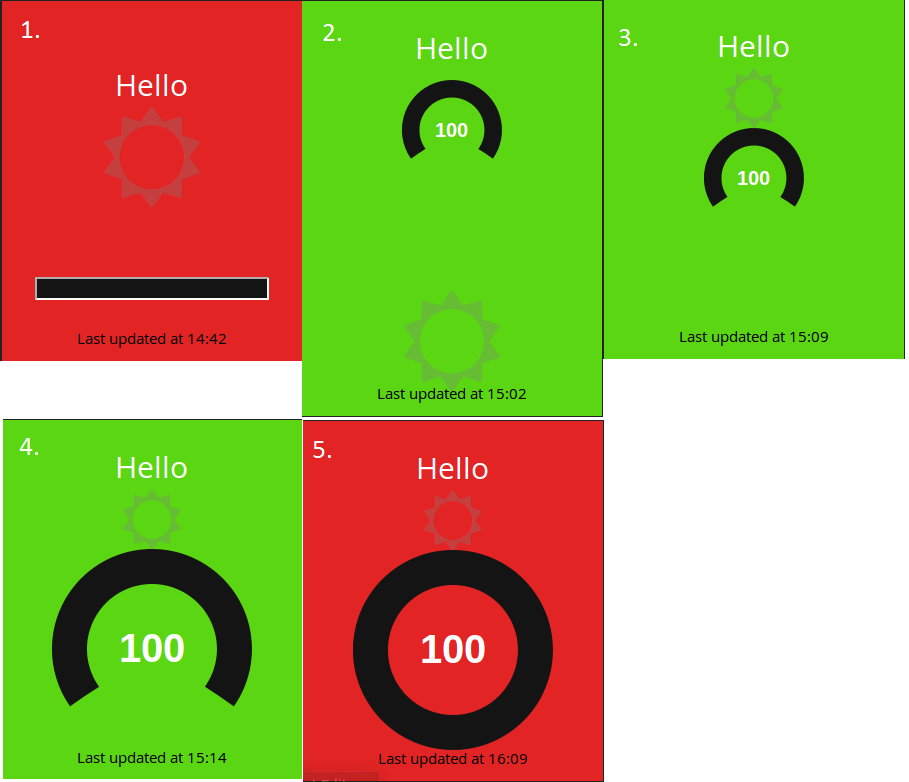
\includegraphics[width=90mm]{proposals.png}
\caption{Voorbeeldwidgets.} 
\label{proposals}
\end{figure} 

\paragraph{Resultaten}
De resultaten zijn te zien in Tabel \ref{results}. Let op, niet iedereen heeft op elk onderdeel geantwoord, daarom zijn er niet op elke vraag 9 antwoorden.

\begin{table}[h!]
\centering
\begin{tabular}{|c|c|c|}
\hline                         										
		 			&	Yes 		&	No		\\	\hline	\hline
Meter				&	8			&	0		\\	\hline
-Large				&	4			&	4		\\	\hline
-On top				&	1			&	6		\\	\hline	
-Circular			&	3			&	5		\\	\hline
Weather report		&	8			&	1		\\	\hline
Background color	&	9			&	0		\\	\hline
\end{tabular}
\caption{Resultaten van de eerste enqu\^ete}
\label{results}
\end{table}

Bijkomende opmerkingen zijn de volgende:
\begin{itemize}
\item "Would combine 1 and 3. Big weather report with small meter at the bottom"
\item "It would be nice if we can show the failure count for failure builds"
\item "I would replace 'last updated' with latest finished build and building since (if in progress). Only show meter when busy building"
\item "Overview of last builds = list or circle with \% of failed/success"
\item "I'd put more visibility for the weather report/more important than current build progress. Maybe also add the date of the last build/number of test or failing tests?"
\end{itemize}

\end{appendices}

\end{document}